\documentclass[
  ukrainian,
  simple,
  floatsection,
]{eskdnaukvd}

%%% Font configuration
\setmainfont{STIX Two Text}
\setsansfont{IBM Plex Sans}
\setmonofont{IBM Plex Mono}
%%%

%%% Math Typesetting
\usepackage{unicode-math}
\setmathfont{STIX Two Math}
%%%

%%% Language configuration
\usepackage{polyglossia}
\setdefaultlanguage{ukrainian}
\setotherlanguage{english}
%%%

%%% List settings
\usepackage{enumitem}
\setlist[enumerate]{
  label*      = {\arabic*.},
  left        = \parindent,
  topsep      = 0\baselineskip,
  parsep      = 0\baselineskip,
  noitemsep, % override itemsep
}
% List settings for levels 2–4
\setlist[enumerate, 2, 3, 4]{
  label*      = {\arabic*.},
  left        = 0em,
  topsep      = 0\baselineskip,
  parsep      = 0\baselineskip,
  noitemsep, % override itemsep
}

\setlist[itemize]{
  label*      = {—},
  left        = \parindent,
  topsep      = 0\baselineskip,
  parsep      = 0\baselineskip,
  itemsep     = 1\baselineskip,
  noitemsep, % override itemsep
}

\setlist[description]{
  font        = {\rmfamily\upshape\bfseries},
  topsep      = 1\baselineskip,
  parsep      = 0\baselineskip,
  itemsep     = 0\baselineskip,
}

\newlist{litlist}{enumerate}{1}
\setlist[litlist]{
  label* = {\arabic*.},
  left = 0em,
}
%%%

%%% Code formatting settings
\newmintinline[minttext]{text}{%
}
%%%

%%% Define width grid
\newlength{\gridunitwidth}
\setlength{\gridunitwidth}{\textwidth / 12}
%%%

%%% GOST strings
\ESKDdepartment{Національний авіаційний університет}
\ESKDclassCode{}
\ESKDtitle{Офісна локальна комп'ютерна мережа}
%\ESKDdocName{Курсова робота}
\ESKDsignature{НАУ 19 2824000 ПЗ}
\ESKDauthor{Клокун~В.\,Д.}
\ESKDtitleApprovedBy{Керівник роботи}{Проценко М.\,М.}
\ESKDchecker{Проценко М.\,М.}
\ESKDcolumnIX{ФККПІ СП-425}
\ESKDapprovedBy{Жуков І.\,А.}
%%%

%%% Define ESKD styles
\ESKDdefaultStyle{nauplain}
%%%

%%% Links and hyperreferences

% Support and define colors
\usepackage{xcolor}
\definecolor{lightblue}{HTML}{03A9F4}
\definecolor{red}{HTML}{F44336}
%

\usepackage{hyperref}
\hypersetup{
  bookmarksnumbered = true,
  colorlinks      = false,
  linkbordercolor = red,
  urlbordercolor  = lightblue,
  pdfborderstyle  = {/S/U/W 1.5},
}
%%%

\begin{document}
  \ESKDthisStyle{empty}

  \begin{titlepage}
  \begin{center}
      Міністерство освіти і науки України\\
      Національний авіаційний університет\\
      % Навчально-науковий інститут комп'ютерних інформаційних технологій\\
      Кафедра комп'ютерних систем та мереж

      \vspace{\fill}
      Курсовий проект\\
      (пояснювальна записка)\\

      \vspace{1 \baselineskip}

      студента 4-го курсу\\
      Інституту комп'ютерних інформаційних технологій\\
      Освітньо-кваліфікаційного рівня «Бакалавр»\\
      Напряму підготовки 6.050102 «Комп'ютерна інженерія»

      \vspace{1 \baselineskip}

      \begin{flushleft}
      Тема: офісна локальна комп'ютерна мережа

      \vspace{2 \baselineskip}

      Виконавець: \hfill Клокун В.\,Д.\\
      Керівник: \hfill Проценко М.\,М.
      \end{flushleft}

      \vspace{\fill}

      Київ 2019
    \end{center}
  \end{titlepage}

  \newpage
  % Fix ESKDX page counter to include the title page
  \setcounter{page}{2}

  \ESKDthisStyle{nausection}
  \tableofcontents

  \section*{Завдання}
    Розробити проект локальної мережі за такими вхідними даними:
    \begin{enumerate}
      \item Серверна кімната~— 107.
      \item Кімнати і кількість робочих станцій у них~(табл.~\ref{tab:task-room-clients}).
      \item Зовнішня~\textenglish{\allcaps{IP}}-адреса~— 178.12.46.115/15.
      \item Пул внутрішніх~\textenglish{\allcaps{IP}}-адрес~— 192.168.56.192/26.
    \end{enumerate}

    \newlength{\tasktabcellwidth}
    \setlength{\tasktabcellwidth}{\columnwidth / 12 - 2 \tabcolsep}
    \begin{table}[!htbp]
      \centering
      \caption{Кімнати та кількість робочих станцій у них}
      \label{tab:task-room-clients}
      \begin{tabular}{
        |*{12}{b{\tasktabcellwidth}|}
      }
        \hline
          108 & 110 & 109 & 111 & 115 & 118 & 120 & 122 & 125 & 128 & 134 & 136 \\
        \hline
          4 & 3 & 4 & 2 & 2 & 6 & 3 & 3 & 3 & 2 & 2 & 2\\
        \hline
      \end{tabular}
    \end{table}

  \section*{Вступ}
  \addcontentsline{toc}{section}{Вступ}
  \ESKDthisStyle{nausection}
    В сучасному світі комп'ютерні мережі дозволяють швидко, зручно і дешево передавати дані на величезні відстані, тому вони стали розповсюдженими засобами обміну даними і використовуються в різноманітних сценаріях:
    \begin{itemize}
      \item у наукових дослідженнях для організації обчислювальних мереж, симуляцій та інформаційної інфраструктуру експериментів;
      \item в індустрії розваг для швидкої доставки контенту;
      \item в медицині для зберігання даних та пошуку інформації щодо захворювань;
      \item у фінансовому секторі для обміну актуальними даними щодо торгів, курсів валют та іншої біржевої інформації, а також організації платежів.
    \end{itemize}
    Отже, видно, що комп'ютерні мережі стали невід'ємною частиною повсякденного життя і професійної діяльності людства.

    Одним зі сценаріїв використання комп'ютерних мереж є їх впровадження в офісах. Організація комп'ютерної мережі в офісі відкриває перед компанією широкий спектр можливостей, а саме:
    \begin{itemize}
      \item співробітникам вивчати актуальну інформацію, яка стосується їх професійної діяльності;
      \item організувати зручний і швидкий обмін даними у рамках компанії;
      \item забезпечити ефективний доступ до цінних внутрішніх ресурсів компанії, зокрема обчислювальних і накопичувальних;
      \item досягти і охопити величезну кількість клієнтів, залишаючись в одній і тій же географічній точці.
    \end{itemize}
    Тобто впровадження локальної комп'ютерної мережі в офісну будівлю є актуальним питанням і необхідною дією, тому у даній курсовій роботі буде розглянутий процес проектування локальної комп'ютерної мережі на прикладі розробки мережі для потреб офісного поверху.

  \clearpage
  \ESKDthisStyle{nausection}
  \section{Основні поняття організації сучасних комп'ютерних мереж}
    \subsection{Метод доступу~\textenglish{\allcaps{CSMA/CD}}}
      У залежності від типу фізичного середовища стандарт~\textenglish{\allcaps{IEEE}}~802.3 має різні модифікації: \textenglish{10Base-5, 10Base-2, 10Base-T, 10Base-F}.

      Для передачі двійкової інформації по кабелю для усіх варіантів фізичного рівня технології \textenglish{Ethernet} використовується манчестерський код.

      Усі різновиди стандартів \textenglish{Ethernet} використовують один і той самий метод доступу до середовища передачі даних, що називається методом колективного доступу з розпізнаванням несучої і виявленням колізій~(\textenglish{carrier sense multiple access with collision detection, \allcaps{CSMA/CD}}).

      Цей метод використовується винятково в мережах із загальною шиною. Усі комп'ютери такої мережі мають безпосередній доступ до загальної шини, тому вона може бути використана для передачі даних між будь-якими двома вузлами мережі. Простота схеми підключення~— це один із факторів, що визначили успіх стандарту \textenglish{Ethernet}. Говорять, що кабель, до якого підключені всі станції, працює в режимі колективного доступу (\textenglish{multiple access, \allcaps{MA}}).

      Усі дані, передані по мережі, розміщуються в кадри визначеної структури і постачаються унікальною адресою станції призначення. Потім кадр передається по кабелю. Усі станції, підключені до кабелю, можуть розпізнати факт передачі кадру і та станція, що упізнає власну адресу в заголовках кадру, записує його вміст у свій внутрішній буфер, обробляє отримані дані і посилає по кабелю кадр-відповідь. Адреса станції-джерела також включена у вихідний кадр, тому станція-одержувач знає, кому потрібно послати відповідь.

      При описаному підході можлива ситуація, коли дві станції одночасно намагаються передати кадр даних по загальному кабелю. Для зменшення імовірності цієї ситуації безпосередньо перед відправленням кадру станція, що передає дані, прослуховує кабель (тобто приймає й аналізує виникаючі на ньому електричні сигнали), щоб виявити, чи не передається вже по кабелю кадр даних від іншої станції. Якщо розпізнається несуча (\textenglish{carrier sense, \allcaps{CS}}), то станція відкладає передачу свого кадру до закінчення чужої передачі, і тільки потім намагається знову його передати.  Але навіть при такому алгоритмі дві станції одночасно можуть вирішити, що по шині в даний момент часу немає передачі, і почати одночасно передавати свої кадри.

      Говорять, що при цьому відбувається колізія, тому що вміст обох кадрів стикається на загальному кабелі, що призводить до перекручування інформації.

      Щоб коректно обробити колізію, усі станції одночасно спостерігають за сигналами, що виникають на кабелі. Якщо передані і одержані сигнали відрізняються, то фіксується виявлення колізії~(\textenglish{collision detection, \allcaps{CD}}).

      Після виявлення колізії станція, що передає, зобов'язана припинити передачу й очікувати протягом короткого випадкового інтервалу часу, а потім може знову зробити спробу передачі кадру.

      З опису методу доступу бачимо, що він має імовірнісний характер, а імовірність успішного одержання в своє розпорядження загального середовища залежить від завантаженості мережі, тобто від інтенсивності виникнення в станціях потреби передачі кадрів. При розробленні цього методу передбачалося, що швидкість передачі даних у 10 Мб/с дуже висока в порівнянні з потребами комп'ютерів у взаємному обміні даними, тому завантаження мережі буде завжди невеликим. Це припущення залишається часто справедливим і зараз, однак тепер існують програми, що працюють у реальному масштабі часу з мультимедійною інформацією, для яких вимагаються набагато вищі швидкості передачі даних. Тому поряд із класичним \textenglish{Ethernet} зростає потреба й у нових високошвидкісних технологіях.

      Метод~\textenglish{\allcaps{CSMA/CD}} визначає основні часові і логічні співвідношення, що гарантують коректну роботу всіх станцій у мережі.

      Між двома послідовно переданими по загальній шині кадрами інформації повинна витримуватися пауза~9{,}6 мкс. Ця пауза потрібна для приведення у вихідний стан мережних адаптерів вузлів, а також для запобігання монопольного захоплення середовища передачі даних однією станцією.

      При виявленні колізії станція видає в середовище спеціальну 32-бітну \textenglish{jam}-послідовність, що підсилює явище колізії для більш надійного розпізнавання її усіма вузлами мережі.

      Після виявлення колізії кожний вузол, що передавав кадр і зіштовхнувся з колізією, після деякої затримки намагається повторно передати свій кадр. Вузол робить максимально 16 спроб передачі цього кадру інформації, після чого відмовляється від його передачі. Розмір затримки вибирається як рівномірно розподілене випадкове число з інтервалу, довжина якого експоненціально збільшується з кожною спробою. Такий алгоритм вибору розміру затримки знижує імовірність колізій і зменшує інтенсивність видачі кадрів у мережу при її високому завантаженні.

      Чітке розпізнавання колізій усіма станціями мережі є необхідною умовою коректної роботи мережі~\textenglish{Ethernet}. Якщо станція, яка передає, не розпізнає колізію і вирішить, що кадр даних нею переданий правильно, тоді цей кадр даних буде загублений, тому що інформація кадру спотвориться через накладення сигналів при колізії, і кадр буде забракований станцією, що його приймає (швидше за все через розбіжність контрольної суми). Звичайно, швидше за все, перекручена інформація буде повторно передана яким-небудь протоколом верхнього рівня, наприклад, транспортним або прикладним, працюючим із установленням з'єднання і нумерацією своїх повідомлень. Але повторна передача повідомлення протоколами верхніх рівнів відбудеться через набагато триваліший інтервал часу (десятки секунд) у порівнянні з мікросекундними інтервалами, якими оперує протокол \textenglish{Ethernet}. Тому якщо колізії не будуть надійно розпізнаватися вузлами мережі \textenglish{Ethernet}, то це призведе до помітного зниження корисної пропускної здатності даної мережі.

      Усі параметри протоколу \textenglish{Ethernet} підібрані таким чином, щоб при нормальній роботі вузлів мережі колізії завжди чітко розпізнавалися. Саме для цього мінімальна довжина поля даних кадру повинна бути не менше ніж 46~байт, що разом із службовими полями дає мінімальну довжину кадру в 72~байти.  Довжина кабельної системи вибирається таким чином, щоб за час передачі кадру мінімальної довжини сигнал колізії встиг би поширитися до самого далекого вузла мережі. Тому для швидкості передачі даних 10~Мб/с, використаної в стандартах \textenglish{Ethernet}, максимальна відстань між двома будь-якими вузлами мережі не повинна перевищувати 2500~метрів.

      Зі збільшенням швидкості передачі кадрів, що має місце в нових стандартах, котрі базуються на тому ж методі доступу \textenglish{\allcaps{CSMA/CD}}, наприклад, \textenglish{Fast Ethernet}, максимальна довжина мережі зменшується пропорційно збільшенню швидкості передачі. У стандарті \textenglish{Fast Ethernet} вона складає 210~м, а в гігабітному \textenglish{Ethernet} обмежена 25 метрами.

      Незалежно від реалізації фізичного середовища, усі мережі \textenglish{Ethernet} повинні задовольняти двом обмеженням, пов'язаним із методом доступу: максимальна відстань між двома будь-якими вузлами не повинна перевищувати 2500~м; у мережі не повинно бути більше ніж 1024~вузлів. Крім того, кожний варіант фізичного середовища додає до цих обмежень свої обмеження, що також повинні виконуватися.

    \subsection{Технологія~«\textenglish{Ethernet}»}
      \textenglish{Ethernet}~— найпопулярніший протокол кабельних комп'ютерних мереж, що працює на фізичному та канальному рівні мережевої моделі \textenglish{\allcaps{OSI}}. Станом на 2016 рік близько 85~\% усіх комп'ютерів у світі були підключені до комп'ютерних мереж по протоколу \textenglish{Ethernet}.

      За строго технічним визначенням \textenglish{Ethernet} — сімейство протоколів стандарту \textenglish{\allcaps{IEEE}} 802.3. \textenglish{Ethernet} тісно пов'язаний з моделлю \textenglish{\allcaps{TCP/IP}}, оскільки у переважній більшості випадків служить для передачі \textenglish{\allcaps{IP}}-пакетів. \textenglish{Ethernet} є найпоширенішім протоколом у сучасних локальних комп'ютерних мережах, також використовується для побудови \textenglish{\allcaps{MAN}} мереж з використанням технології \textenglish{Metro Ethernet}.

      \textenglish{Ethernet} було спроектовано згідно з технологією \textenglish{\allcaps{CSMA/CD}} (множинний доступ з контролем несучої та виявленням колізій). Хоча з широким застосуванням мережевих комутаторів та засобу передачі повний дуплекс проблема виникнення колізій в мережах \textenglish{Ethernet} майже не зустрічається.

      \textenglish{Ethernet}-мережі працюють на швидкостях 10Мбіт/с, \textenglish{Fast Ethernet} — на швидкостях 100Мбіт/с, \textenglish{Gigabit Ethernet} — на швидкостях 1000Мбіт/с, \textenglish{10 Gigabit Ethernet} — на швидкостях 10Гбіт/с. В кінці листопада 2006 року було прийняте рішення про початок розробок наступної версії стандарту з досягненням швидкості 100Гбіт/с (\textenglish{100 Gigabit Ethernet}).

      Вдосконалення мережних засобів, зокрема адаптерів, дало змогу широко застосовувати виту пару як середовище передавання. В рамках стандарту \textenglish{Ethernet} створені специфікації \textenglish{10BaseT}, що використовує дві неекрановані виті пари \textenglish{\allcaps{UTP} (Unshielded Twisted Pair)} 3, 4 або 5 категорій, та \textenglish{100BaseT4}, що ґрунтується на чотирьох витих парах \textenglish{\allcaps{UTP}} 5 категорії або екранованій витій парі \textenglish{\allcaps{STP} (Shielded Twisted Pair)}. Для зв'язку між вузлами мережі необхідними є дві виті пари провідників: одна — для передавання, інша — для приймання інформації. Звичайно, замість двох кабелів по одній парі витих провідників у кожній використовують один кабель з чотирма парами провідників. Окрім економії та технічних переваг, це створює можливість переходу на більш швидкісні мережні архітектури без заміни самого кабелю.

    \subsection{Формат кадру~\textenglish{Ethernet}}
      Кадр~\textenglish{Ethernet}~— це фрагмент даних протоколу канального рівня, який використовує механізми нижчого фізичного рівня~\textenglish{Ethernet}. Інакше кажучи, фрагмент даних в~\textenglish{Ethernet}-з'єднанні переносить \textenglish{Ethernet}-кадр як своє корисне навантаження. Існує декілька форматів Ethernet-кадру~(рис.~\ref{fig:ethernet-frames}):
      \begin{itemize}
        \item Первинний \textenglish{Version I} (більше не застосовується).
        \item \textenglish{Ethernet Version 2} або \textenglish{Ethernet}-кадр~II, ще званий \textenglish{\allcaps{DIX}} (абревіатура перших букв фірм-розробників \textenglish{\allcaps{DEC}, Intel, Xerox})~— найпоширена і використовується до сьогодні. Часто використовується безпосередньо протоколом інтернет.
        \item \textenglish{Novell} — внутрішня модифікація \textenglish{\allcaps{IEEE}} 802.3 без \textenglish{\allcaps{LLC} (Logical link control)}.
        \item Кадр \textenglish{\allcaps{IEEE} 802.2 \allcaps{LLC}}.
        \item Кадр \textenglish{\allcaps{IEEE} 802.2 \allcaps{LLC/SNAP}}.
      \end{itemize}

      \begin{figure}[!htbp]
        \centering
        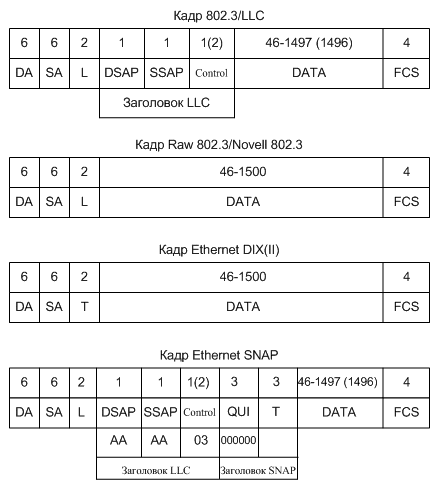
\includegraphics[height = 12\baselineskip]{./assets/00-01-ethernet-frames.png}
        \caption{Різні формати кадрів~\textenglish{Ethernet}}
        \label{fig:ethernet-frames}
      \end{figure}

      Деякі мережеві карти \textenglish{Ethernet}, що випускались компанією \textenglish{Hewlett-Packard}, використовували при роботі кадр формату \textenglish{\allcaps{IEEE} 802.12}, відповідно стандарту \textenglish{100VG-AnyLAN}.

      Як доповнення Ethernet-кадр може містити тег \textenglish{\allcaps{IEEE} 802.1Q} для ідентифікації \textenglish{\allcaps{VLAN}}, до якої він адресований, і \textenglish{\allcaps{IEEE} 802.1p} для вказання пріоритету.

      Різні типи кадру мають різний формат і значення \textenglish{\allcaps{MTU}}.

      Кадр починається з преамбули яка має розмір 8 байт (64 біт) і складається з послідовності «10», повтореної 31 раз, та «11» у кінці.

      Далі йде адреса отримувача і адреса відправника які займають по 6 байт кожна. Якщо адреса отримувача починається з 1, то це групова передача (multicast) (всі в групі). Якщо адреса отримувача складається з самих одиниць (FF:FF:FF:FF:FF:FF) — це широкомовна передача (broadcast). Для групової передачі треба налаштовувати групи, тому вона використовується рідко.

      Наступне поле — тип, або довжина, залежно від того, до якого стандарту належить кадр. З історичних причин, якщо значення в полі менше за 0x600 = 1536, то це довжина, а якщо більше — тип, який визначає, якому протоколу мережевого рівня передати кадр, якщо з \textenglish{Ethernet} працює кілька мережевих протоколів. 0x800 — IPv4. Якщо тип не вказано, то що робити з кадром визначає протокол \textenglish{Logical link control}, це ще 8 байт заголовків.

      Далі йде поле даних, менше за 1500 байт, але більше за 46 байт.

      Якщо даних менше за 46 байт, після них додається наповнювач (\textenglish{pad}) потрібного розміру. Це потрібно щоб кадр можна було відрізнити від сміття в каналі, яке з'являється коли передача припиняється при виявленні колізії, і щоб кадр був достатньо довгим аби не передатись повністю до того як колізія виявиться.

      Останнє поле — контрольна сума. Це 32-х бітний \textenglish{\allcaps{CRC}}. При виявленні помилки кадр видаляється.

  \section{Топологія мережі}
  \ESKDthisStyle{nausection}
    Необхідно розробити проект офісної локальної комп'ютерної мережі для заданого поверху будівлі~(рис.~\ref{fig:floor-plan}).

    \begin{figure}[!htbp]
      \centering
      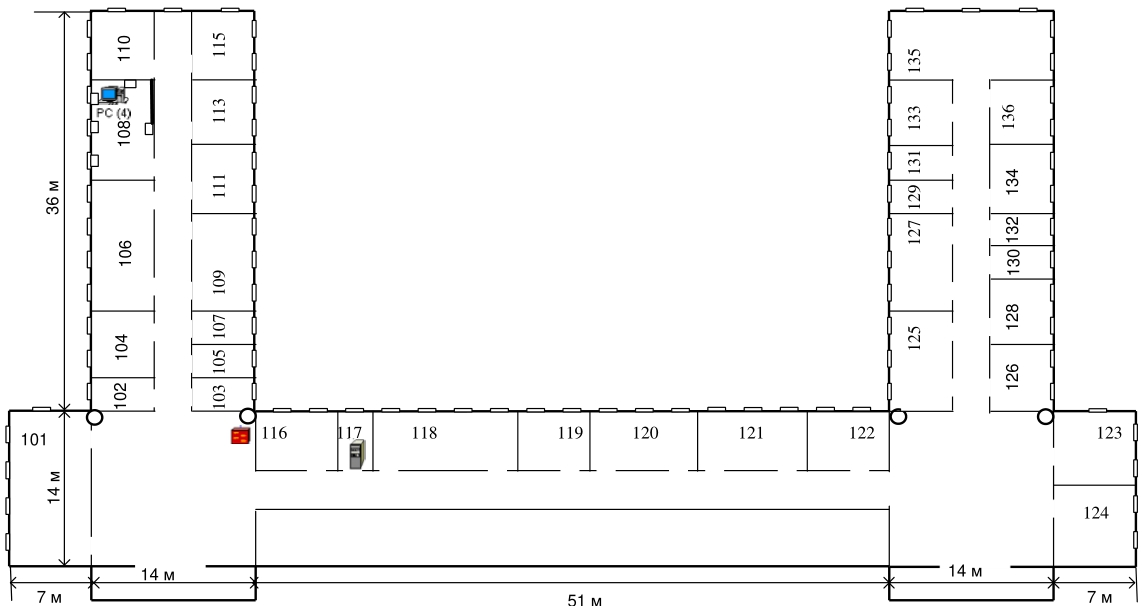
\includegraphics[width = \columnwidth]{./assets/01-floor-plan.jpg}
      \caption{План цільового поверху, для якого необхідно спроектувати локальну комп'ютерну мережу}
      \label{fig:floor-plan}
    \end{figure}

    Також проект має задовольняти мінімальні вимоги до кількості клієнтів~(табл.~\ref{tab:room-clients}), а також вимоги реалізації, а саме:
    \begin{itemize}
      \item серверна кімната має знаходитись в кімнаті~107;
      \item необхідно створити 3 віртуальні локальні мережі~(\textenglish{\allcaps{VLAN}});
      \item розмістити 2~фізичні сервери для накопичення та зберігання даних;
      \item запропонувати рішення щодо встановлення каналу зв'язку з провайдером~\textenglish{Internet}, розподілу~\textenglish{IP}-адрес та трансляції адрес;
      \item передбачити заходи із захисту мережі.
    \end{itemize}
    Розробка проекту починається з вибору топології, і поставлені обмеження дозволяють краще її підібрати.

    \newlength{\tmptabcellwidth}
    \setlength{\tmptabcellwidth}{\columnwidth / 12 - 2 \tabcolsep}
    \begin{table}[!htbp]
      \centering
      \caption{Кімнати та кількість робочих станцій у них}
      \label{tab:room-clients}
      \begin{tabular}{
        |*{12}{b{\tmptabcellwidth}|}
      }
        \hline
          108 & 110 & 109 & 111 & 115 & 118 & 120 & 122 & 125 & 128 & 134 & 136 \\
        \hline
          4 & 3 & 4 & 2 & 2 & 6 & 3 & 3 & 3 & 2 & 2 & 2\\
        \hline
      \end{tabular}
    \end{table}

    \subsection{Вибір топології мережі}

      Враховуючи сформульовані умови і обмеження, топологія, обрана для проектування, має вирішувати такі задачі:
      \begin{itemize}
        \item підтримувати надійність мережі, тобто організувати середовище, в якому несправність одного клієнта якнайменш вплине на інших клієнтів;
        \item сегментувати мережу, тобто розподілити її на менші логічні і структурні одиниці;
        \item задати центральну точку для обміну даними та підключення до інфраструктури провайдера.
      \end{itemize}
      Щоб вирішити такий широкий спектр поставлених задач, для розробки проекту офісної локальної комп'\-ю\-тер\-ної мережі була обрана гібридна топологія~— така топологія, яка поєднує в собі декілька стандартних топологій.

      Щоб задати центральну точку обміну даними та підключення до інфраструктури провайдера, добре підходить топологія~«Зірка»~(рис.~\ref{fig:topology-star}).

      \begin{figure}[!htbp]
        \centering
        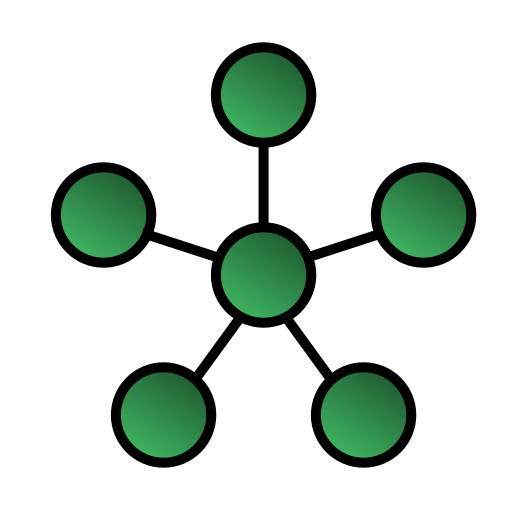
\includegraphics[width = 4 \gridunitwidth]{./assets/02-topology-star.png}
        \caption{Приклад топології~«Зірка»}
        \label{fig:topology-star}
      \end{figure}

      «Зірка» передбачає, що всі точки-клієнти під'єднуються до центральної точки, яка в свою чергу розподіляє і перенаправляє повідомлення між клієнтами або ж повторює повідомлення усім під'єднаним клієнтам. Наявність центральної точки у топології~«Зірка» суттєво збільшує надійність мережі, адже якщо вийде з ладу канал передачі даних між двома точками, лише одна з них буде ізольована від мережі, тобто несправність однієї точки чи каналу обміну даними мінімально вплине на інші клієнти. Однак, топологія «Зірка» має суттєвий недолік~— єдину точку відмови: якщо у топології відмовить центральна точка, вся мережа перестане працювати. Тим не менш, сучасні проектно-технічні засоби на кшталт надійного обладнання, обмеження фізичного доступу та застосування надлишковості дозволяють впоратись з цим недоліком, тому топологія~«Зірка» буде основною структурною одиницею топології розроблюваної мережі.

      Щоб з'єднати структурні сегменти мережі, що проектується, необхідно передбачити можливість підключення усіх існуючих сегментів мережі, а також зручного додавання сегментів у майбутньому. Для цього зручно скласти найменші структурні сегменти в таку ієрархію, в якій найнижчі кінцеві сегменти підключаються до вищих, розподіляючих сегментів, а вищі розподіляючі сегменти~— до ще вищих, і таким чином аж до кореневого вузла доступу, який буде підключений до мережі «Інтернет» через інфраструктуру провайдера.

      Якщо для прикладу розглянути сегменти-«Зірки» як єдиний вузол, такий ієрархічний спосіб під'єднання нагадує топологію «Шина»~(рис.~\ref{fig:topology-bus}), і тому з'єднання сегментів таким способом дозволить підключити усі сегменти одне до одного, а також зручно додавати нові сегменти у майбутньому.

      \begin{figure}[!htbp]
        \centering
        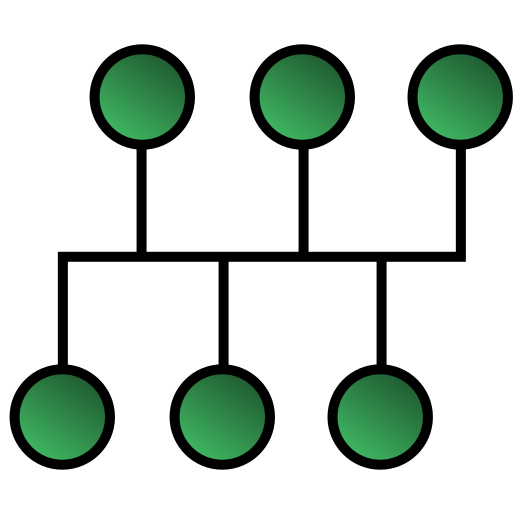
\includegraphics[width = 4 \gridunitwidth]{./assets/03-topology-bus.png}
        \caption{Приклад топології~«Шина»}
        \label{fig:topology-bus}
      \end{figure}

      Отже, необхідна гібридна топологія поєднає у собі властивості стандартних топологій «Зірка» та «Шина». Це поєднання називається деревовидною топологією~(рис.~\ref{fig:tree-topology}).

      Деревовидна топологія є конкретною реалізацією поняття дерева з теорії графів, в якому перший вузол дерева прийнято називати коренем, наступні вузли високих рівнів~— батьками, а низьких рівнів~— дітьми.

      \begin{figure}[!htbp]
        \centering
        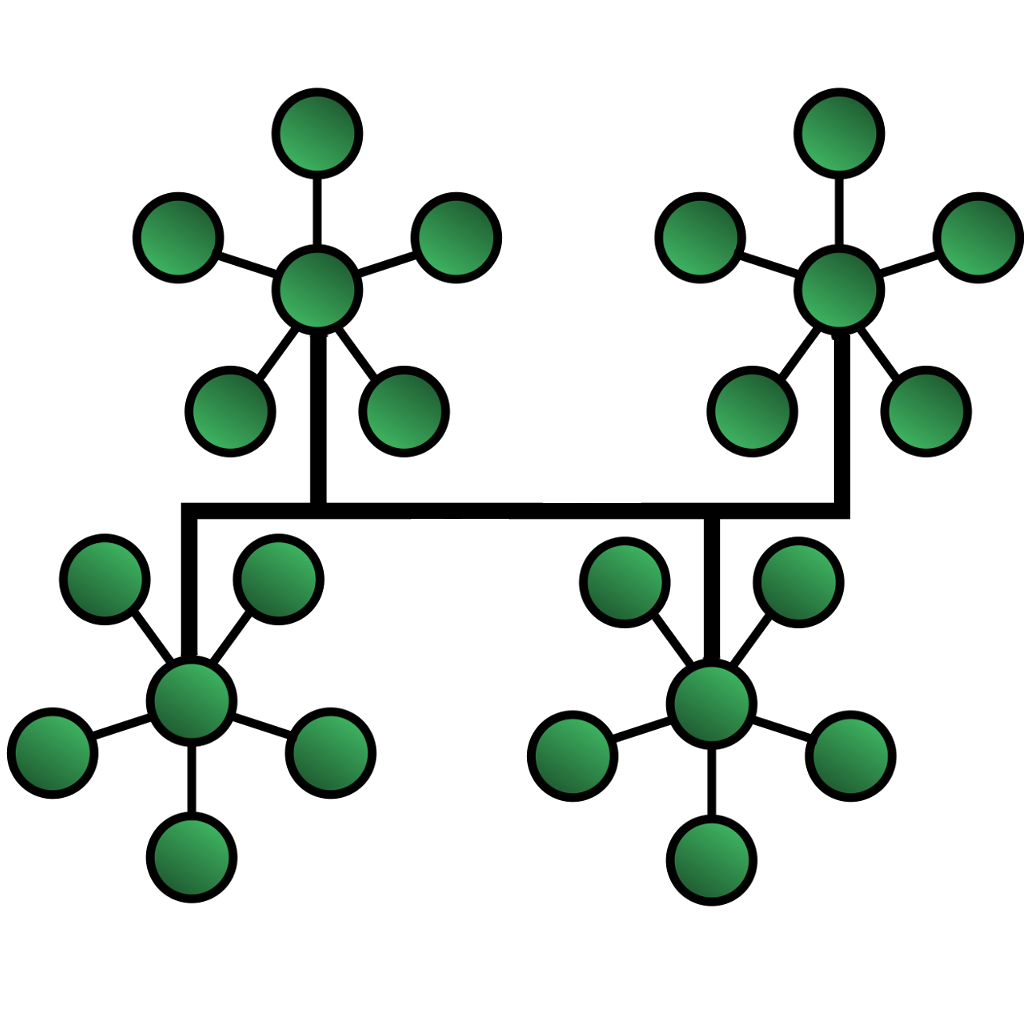
\includegraphics[width = 8 \gridunitwidth]{./assets/04-topology-tree.png}
        \caption{Приклад деревовидної топології}
        \label{fig:tree-topology}
      \end{figure}

      Отже, в результаті вибору була обрана гібридна деревовидна топологія, яка дозволить зручно вирішити задачі і задовольнити вимоги, поставлені до потрібної мережі: забезпечити надійність мережі, сегментувати її, а також організувати центральну точку підключення до провайдера і обміну даними.

    \subsection{Реалізація обраної топології}
      Обравши зручну і ефективну топологію для проекту комп'ютерної мережі, необхідно спроектувати план її втілення. Для цього, перш за все, необхідно скласти перелік обладнання, яке знадобиться для розробки мережі, врахувавши потреби мережі.

      Цільова мережа має підтримувати одночасну роботу не менш ніж 36 робочих станцій різного призначення, а також 2 сервери. Робочі станції повинні бути об'єднані у 3~віртуальні локальні мережі. Щоб задовольнити цю потребу, необхідно використовувати маршрутизатори рівня 2 моделі~\textenglish{\allcaps{OSI}}, які дозволять використати технологію~\textenglish{\allcaps{IEEE}~802.1q}, щоб реалізувати розподіл на віртуальні мережі.

      Враховуючи, що передбачається робота приблизно 36~робочих станцій, а також той факт, що будівля складається з декількох крил, щоб розмістити користувачів у мережі, потребується 2 24-портових комутатори. Також хорошою практикою при реалізації топології є винесення серверів в окрему мережу, що буде реалізовано за допомогою технології віртуальних локальних мереж, але щоб підкреслити можливість розширення мережі і подальше огородити сервери, використаємо для них окремий комутатор. Отже, знадобиться 3 комутатори рівня 2, які будуть комутаторами рівня доступу.

      Оскільки проектована мережа має надавати можливість розширення, підтримувати швидку роботу багатьох робочих станцій з мережею~«Інтернет», а також надавати стабільний і миттєвий доступ до ресурсів двох серверів всередині мережі, доцільно використати пристрій рівня розподілу. Щоб економно організувати високу швидкість обміну даними всередині мережі, варто використати комутатори рівня~3: вони коштують значно дешевше за маршрутизатори аналогічної швидкодії, підтримують всі технології, які можуть знадобитись при організації внутрішньої мережі, а також надають можливість зручного розширення, дозволяючи лише увімкнути новий комутатор рівня~2 і під'єднувати до нього нові клієнти.

      Локальна офісна комп'ютерна мережа, що проектується, передбачає доступ до мережі «Інтернет». Щоб працювати з мережею мережею~«Інтернет», а тим паче від імені 36 клієнтів внутрішньої мережі, необхідно маршрутизувати і перетворювати трафік, який приходить зовні та генерується всередині. Для цього знадобиться маршрутизатор.

      Отже, щоб реалізувати обрану топологію, необхідно таке обладнання:
      \begin{itemize}
        \item Маршрутизатор.
        \item Комутатор рівня 3.
        \item Комутатори рівня 2.
      \end{itemize}
      При реалізації мережі необхідно знати, яке конкретне обладнання варто використовувати, тому необхідно визначити зручні і доцільні конкретні пристрої.

      Так як для моделювання мережі використовується програма~\textenglish{Cisco Packet Tracer}, то для реалізації мережі буде використане обладнання фірми~\textenglish{Cisco}. Судячи з поставлених вимог, мережа проектується для потреб малого або середнього бізнесу з перспективами зростання або сегменту кампусної мережі, тому під час вибору будуть розглядатись пристрої саме цієї ніші.

      Для реалізації найнижчого рівня топології мережі~— рівня доступу~— необхідно три 24-портових комутатори рівня~2. Серед обладнання, доступного в середовищі~\textenglish{Packet Tracer}, найкраще підходять комутатори~\textenglish{Cisco Catalyst 2960-24TT} вони мають 24 порти, підтримують технологію~\textenglish{\allcaps{IEEE}~802.1q}, яка дозволить призначити їх портам бажані віртуальні локальні мережі, тому вони стануть комутаторами рівня доступу, до яких будуть підключатись кінцеві клієнти: робочі станції і сервери.

      Щоб організувати рівень розподілу, вистачить одного пристрою~— комутатора рівня~3, а саме \textenglish{Cisco Catalyst 3560}. Цей комутатор відповідатиме за об'єднання комутаторів рівня доступу, і оскільки він має 24 порти, мережа може бути відчутно розширена. Висока швидкодія комутатора дозволить ефективно маршрутизувати трафік всередині мережі. Крім цього, обраний комутатор підтримує роботу з протоколом~\textenglish{\allcaps{DHCP}}, тому буде виділяти \textenglish{\allcaps{IP}}-адреси клієнтам внутрішньої мережі.

      В рамках задачі доступ до мережі «Інтернет» організується за допомогою інфраструктури провайдера. Провайдер надає офісу виділений канал зв'язку за допомогою технології~\textenglish{Fiber-to-the-x~(\allcaps{FTT}x)}: до будівлі ведеться оптоволоконний кабель, а підключення внутрішніх клієнтів будівлі, тобто термінація на останній милі, виконується за допомогою витої пари.

      Враховуючи задані параметри підключення провайдера і проектованої мережі, серед доступних машрутизаторів доцільно використати~\textenglish{Cisco Catalyst 2911}. Ця модель надає можливість підключення за технологією~\textenglish{Gigabit Ethernet}, а також трансляцію мережевих адрес за допомогою технології~\textenglish{Network Address Translation~(\allcaps{NAT})}, необхідну, щоб клієнти внутрішньої мережі офісу могли працювати із мережею~«Інтернет». Також даний маршрутизатор надає широкий набір можливостей роботи з безпекою: апаратне прискорення технологій шифрування, які використовуються для~\textenglish{\allcaps{VPN}}, і управління обліковими записами за допомогою автентифікації, авторизації та обліку~(\textenglish{authentication, authorization and accounting, \allcaps{AAA}}).

      Щоб змоделювати інфраструктуру провайдера, яка використовується для доступу до мережі «Інтернет», буде використана комбінація аналогічного маршрутизатора~\textenglish{Cisco Catalyst 2911} і підключеного до нього публічного сервера.

      Отже, після вибору конкретних пристроїв, була побудована логічна топологія офісної локальної комп'ютерної мережі~(рис.~\ref{fig:net-topology-logical}).

      \begin{figure}[!htbp]
        \centering
        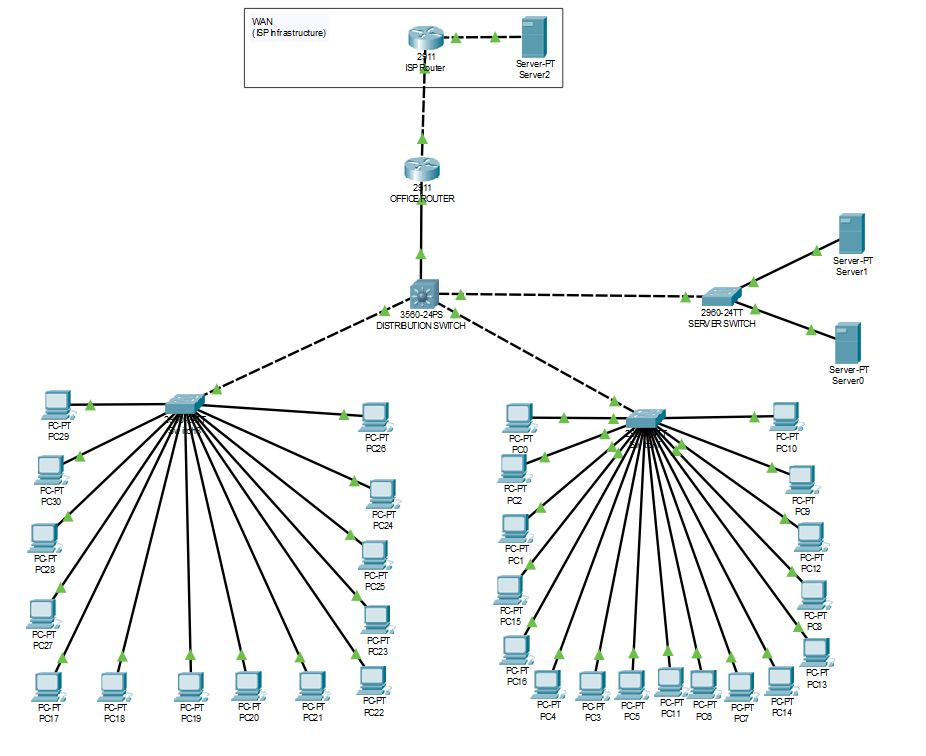
\includegraphics[width = \columnwidth]{./assets/05-net-topology-logical.png}
        \caption{Логічна топологія для проектованої офісної мережі}
        \label{fig:net-topology-logical}
      \end{figure}

  \section{Налаштування мережі}
  \ESKDthisStyle{nausection}
    Після створення логічної топології можна переходити до проектування її фізичної реалізації. Враховуючи особливості будівлі, обраної топології і обладнання, був розроблений проект фізичної реалізації топології офісної локальної комп'ютерної мережі~(рис.~\ref{fig:net-topology-physical}).

      \begin{figure}[!htbp]
        \centering
        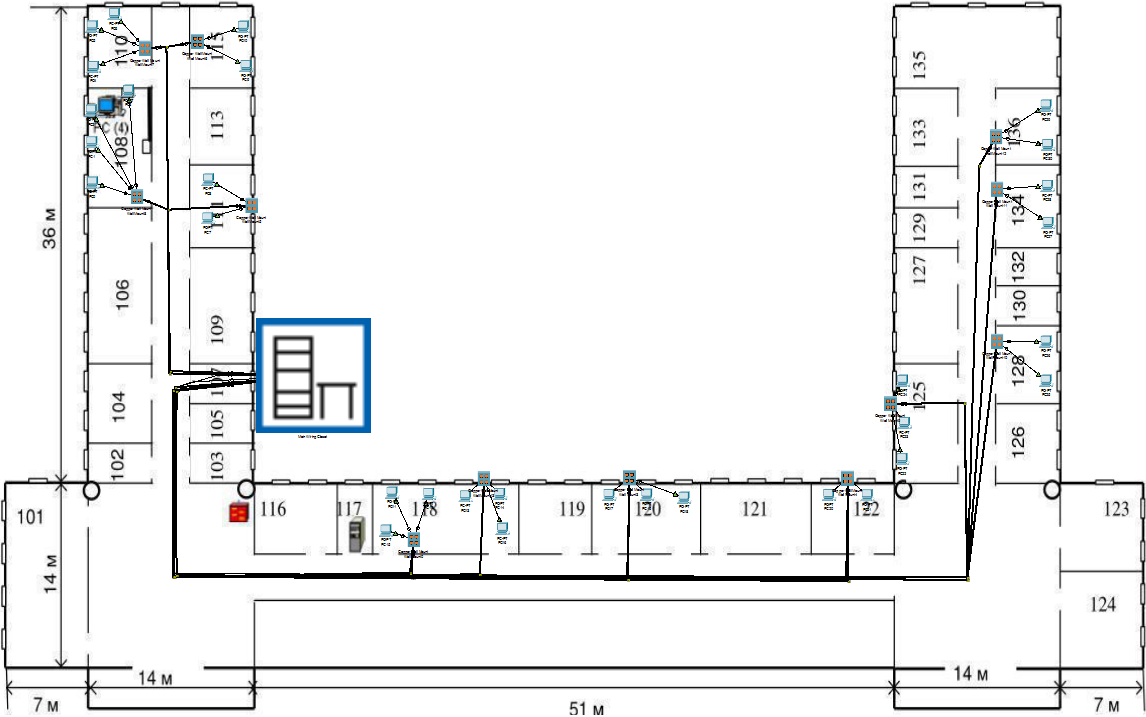
\includegraphics[width = \columnwidth]{./assets/06-net-topology-physical.png}
        \caption{Фізична топологія для проектованої офісної мережі}
        \label{fig:net-topology-physical}
      \end{figure}

    \subsection{Розміщення мережевого обладнання}
      У розробленому проекті офісної мережі передбачено, що мережеве обладнання розміщується у спеціально виділеній стійці~(рис.~\ref{fig:wiring-closet}), яка знаходиться в кімнаті~107. На жаль, через технічні обмеження програми~\textenglish{Cisco Packet Tracer}, неможливо зменшити розмір стійки так, щоб він підійшов до розмірів плану поверху, тому схематично вона знаходиться за межами потрібної кімнати.

      Використання окремої стійки дозволяє покращити безпеку у мережі, оскільки доступ до серверної кімнати і стійки повинні мати виключно авторизовані і кваліфіковані сторони, а також зручність для кінцевих користувачів: їм не заважатиме шум та тепло, які виділяються під час роботи обладнання. Також використання окремої серверної кімнати і стійки дає можливість організувати спеціальні умови для відведення тепла і пожежної безпеки.

      \begin{figure}[!htbp]
        \centering
        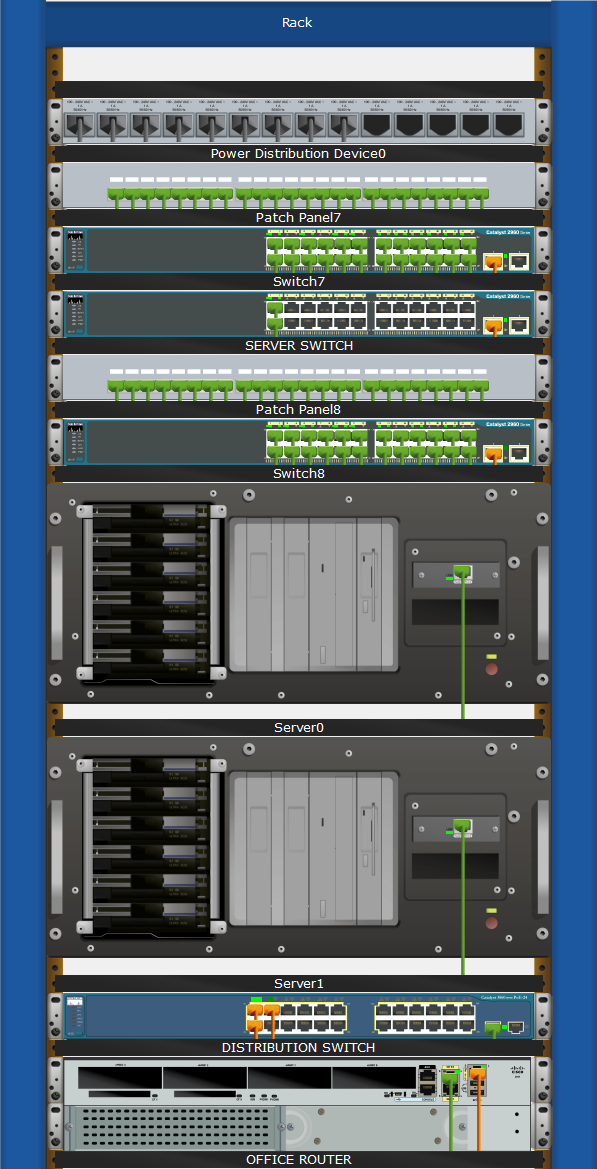
\includegraphics[width = 6 \gridunitwidth]{./assets/07-wiring-closet-04.png}
        \caption{Стійка з мережевим обладнанням}
        \label{fig:wiring-closet}
      \end{figure}

      Всередині стійки міститься все обладнання, необхідне для роботи мережі, а саме:
      \begin{itemize}
        \item Пристрій живлення.
        \item Патч-панелі.
        \item Офісний маршрутизатор, підключений до мережі інтернет.
        \item Комутатор рівня розподілу.
        \item Комутатори рівня доступу.
        \item Два сервери для накопичення і зберігання файлів.
      \end{itemize}
      Також, заради симуляції доступу до мережі~«Інтернет», всередині стійки розташований маршрутизатор і сервер провайдера, але в реальних умовах вони знаходяться в інфраструктурі провайдера.

    \subsection{Особливості укладення кабеля}
      Як видно на реалізації логічної топології~(рис.~\ref{fig:net-topology-logical}), у ній використовуються різні з'єднання, тобто деякі пристрої з'єднані за допомогою різних кабелів. Це зумовлено тим, що незважаючи на здатність сучасних мережевих інтерфейсів автоматично підключатись одне до одного за допомогою будь-яких типів з'єднуючих кабелів, програма~\textenglish{Cisco Packet Tracer} вимагає строгого дотримання правил прокладки кабелів: щоб з'єднати пристрої різних типів, необхідно використовувати прямий кабель, а пристрої одного типу~— перехресний кабель. Тому для підключення кінцевих клієнтів до комутаторів рівня~2, а також комутатора рівня~3 до маршрутизатора використовується прямий кабель «вита пара», тоді як для підключення комутаторів рівня~2 до комутатора рівня~3, а також офісного маршрутизатора до маршрутизатора провайдера використовується перехресний кабель «вита пара».

      Укладення кабеля всередині будівлі виконується у фальшстелі~— спеціальному просторі між реальною стелею та зовнішніми підвісними панелями, призначеному для розміщення кабелів у ньому. Такий спосіб проведення кабеля є найзручнішим для початкової установки і обслуговування мережевої інфраструктури, адже мережевий інженер матиме зручний доступ до будь-якої ділянки маршруту у будь-який час.

      Кабель укладається за чіткими принципами:
      \begin{itemize}
        \item Основне мережеве обладнання підключається до патч-панелі.
        \item Від патч-панелі починається проведення кабелів до кінцевих клієнтів.
        \item На початку кабелі виводяться в сторону магістральних ділянок~— областей у фальшстелі, які знаходяться приблизно посередині коридору.
        \item Дійшовши до магістральної ділянки, кабелі заводяться у магістральний кабель-канал, який захищає прокладений кабель від механічних пошкоджень, а також зменшує рівень зовнішніх завад.
        \item Наближаючись до цільової ділянки, де знаходиться точка, з якої необхідно організувати доступ до мережі, кабель виводиться з магістрального кабель-каналу у напрямку точки доступу.
        \item Кабель прокладається до кінцевої \textenglish{Ethernet}-розетки доступу~(рис.~\ref{fig:wall-outlets}).
        \item Клієнти підключаються до розетки за допомогою власних патч-кордів.
      \end{itemize}
      Дотримання вищезазначених принципів дозволить краще структурувати кабельне розведення всередині приміщення, запобігти непотрібному пошкодженню його конструкцій, а також дати можливість зручної зміни кількості клієнтів у майбутньому, підключаючи або відключаючи їх від розеток доступу або встановлюючи нові розетки.

      \begin{figure}[!htbp]
        \centering
        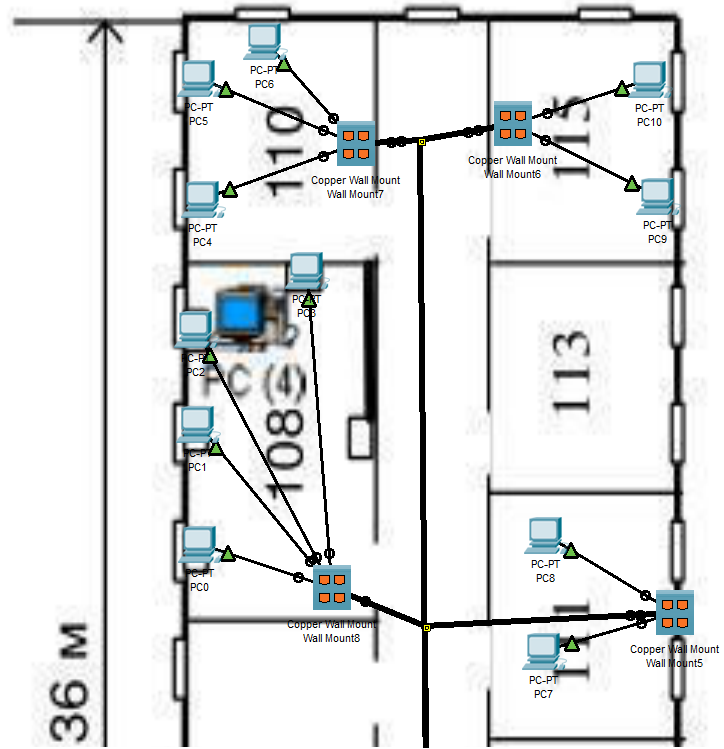
\includegraphics[width = 6 \gridunitwidth]{./assets/08-wall-outlets.png}
        \caption{Розташування деяких розеток доступу до мережі}
        \label{fig:wall-outlets}
      \end{figure}

    \subsection{Налаштування мережевого обладнання}

      \subsubsection{Поділ на~\textenglish{\allcaps{VLAN}} і розподіл~\textenglish{\allcaps{IP}}-адрес}

      Монтаж необхідної мережевої інфраструктури дозволить почати розгортання самої мережі. Щоб розпочати розгортання, необхідно розподілити існуючі ресурси мережі і налаштувати мережеве обладнання.

      Розподіл мережевих ресурсів починається з аналізу налаштувань. До налаштувань, які будуть використані для проекту офісної локальної комп'ютерної мережі, поставлені такі вимоги:
      \begin{enumerate}
        \item Розподілити локальну мережу на три віртуальні мережі~(\textenglish{\allcaps{VLAN}}).
        \item Зовнішня~\textenglish{\allcaps{IP}}-адреса мережі~— 178.12.46.15/15.
        \item Пул внутрішніх~\textenglish{\allcaps{IP}}-адрес~— 192.168.56.192/26.
      \end{enumerate}
      Враховуючи поставлені вимоги, перш за все необхідно розпочати з розподілу локальної мережі на менші віртуальні локальні мережі.

      У проекті передбачено, що мережа складатиметься з 36 робочих станцій і 2~серверів. Хорошою практикою для створення безпечного середовища у мережі є виділення серверів у окрему віртуальну мережу, тому є необхідність у як мінімум двої віртуальних мережах. Розподіливши пул доступних~\textenglish{\allcaps{IP}}-адрес навпіл, як це можливо за протоколом~\textenglish{\allcaps{IP}}, користувачам не вистачить адрес у новоутворених пулах, тому необхідно розподілити один з пулів ще раз, прийшовши до потрійного розподілу~(табл.~\ref{tab:inner-ip-pool-segmentation}).

      \begin{table}[!htbp]
        \centering
        \caption{Розподіл пулу внутрішніх~\textenglish{\allcaps{IP}}-адрес}
        \label{tab:inner-ip-pool-segmentation}
        \begin{tabular}{
          |v{6 \gridunitwidth - 2 \tabcolsep}
          |n{3 \gridunitwidth - 2 \tabcolsep}
          |n{3 \gridunitwidth - 2 \tabcolsep}
          |
        }
          \hline
            Призначення & Доступні адреси & Підмережа \\
          \hline
            Перша частина користувачів & 30 & 192.168.56.192/27 \\
            Друга частина користувачів & 12 & 192.168.56.224/28 \\
            Сервери і мережеве обладнання & 12 &  192.168.56.240/28 \\
          \hline
        \end{tabular}
      \end{table}

      Після розподілу внутрішніх~\textenglish{\allcaps{IP}}-адрес, можна поставити їм у пряму відповідність віртуальні локальні мережі. Визначення віртуальних локальних мереж відбувається на портах комутаторів, тому необхідно пам'ятати, які комутатори для чого призначені, і для чого будуть використовуватись їх порти. Наприклад, два з необхідних комутаторів рівня доступу призначені для кінцевих користувачів. Це 24-портові комутатори, тому сумарна кількість портів, які вони надають, менша за кількість доступних внутрішніх~\textenglish{\allcaps{IP}}-адрес, призначених користувачам. Тим не менш, ці комутатори не призначені для використання іншим обладнанням, а також вони знаходяться у безпечному місці, тому доцільно пов'язати усі порти кожного з комутаторів до віртуальних мереж~1 і 2 відповідно.

      Залишається третій комутатор рівня доступу, до якого будуть підключатись сервери. Сервери виділяються в окрему віртуальну мережу~— \textenglish{\allcaps{VLAN}}~3. Отже, отримали схему розподілу портів за віртуальними мережами.

      \begin{table}[!htbp]
        \centering
        \caption{Розподіл портів мережевого обладнання за віртуальними мережами~\textenglish{\allcaps{VLAN}}}
        \label{tab:vlan-segmentation}
        \begin{tabular}{
          |v{5 \gridunitwidth - 2 \tabcolsep}
          |v{3 \gridunitwidth - 2 \tabcolsep}
          |n{2 \gridunitwidth - 2 \tabcolsep}
          |n{2 \gridunitwidth - 2 \tabcolsep}
          |
        }
          \hline
            Призначення~\textenglish{\allcaps{VLAN}} & Комутатор & Порти & №~\textenglish{\allcaps{VLAN}} \\
          \hline
            Перша група користувачів      & \textenglish{Switch7}       & 1–24 & 1 \\
            Друга група користувачів      & \textenglish{Switch8}       & 1–24 & 2 \\
            Сервери і мережеве обладнання & \textenglish{Server Switch} & 1–24 & 3 \\
          \hline
        \end{tabular}
      \end{table}

    \subsubsection{Налаштування комутаторів рівня доступу}
      Після розподілу мережевих ресурсів, а саме~\textenglish{\allcaps{IP}}-адрес між клієнтами, а також визначення віртуальних локальних мереж~\textenglish{\allcaps{VLAN}}, необхідно налаштувати мережеве обладнання. Найзручніше перевіряти коректність налаштувань починаючи з найнижчого рівня логічної ієрархії в топології, тобто з комутаторів рівня доступу, тому треба виконати їх налаштування~(лістинг~\ref{lst:switch-l2-vlans}).

      \begin{listingplaintext}{Створення віртуальних локальних мереж на комутаторі рівня доступу}{lst:switch-l2-vlans}
        en
        conf t
        # Створити VLAN номер 2
        vlan 2
        # Дати створеній VLAN ім'я «USERS»
        name USERS01
        # Обрати інтерфейси Fast Ethernet від 1 до 24
        int range fa0/1-24
        # Встановити їх у режим доступу
        switchport mode access
        # Дозволити їм передавати пакети, відмічені як для VLAN 2
        switchport acccess vlan 2
      \end{listingplaintext}

      Після виконання вищезазначених команд усі порти комутатора, на якому вони виконувались, будуть позначені як порти~\textenglish{\allcaps{VLAN}}~2. Щоб виділити віртуальні мережі на інших комутаторах, необхідно виконати аналогічні команди, вказуючи лише номер та назву необхідної~\textenglish{\allcaps{VLAN}}.

      Однак, крім виділення портів під необхідні віртуальні мережі, необхідно забезпечити можливість обміну даними між різними створеними~\textenglish{\allcaps{VLAN}}, тобто дозволити прийом даних з усіх створених віртуальних мереж на усіх комутаторах~(лістинг~\ref{lst:switch-l2-trunk}).

      \begin{listingplaintext}{Налаштування комутатора рівня доступу на прийом даних з усіх створених віртуальних мереж}{lst:switch-l2-trunk}
        # Обрати інтерфейс Gigabit Ethernet 0/1
        int gi0/1
        # Встановити режим транкінгу (об'єднання в пучок)
        switchport mode trunk
        # Дозволити в пучку VLAN 2–4
        switchport trunk allowed vlan 2-4
        end
        # Зберегти конфігурацію
        wr mem
      \end{listingplaintext}
      Тепер комутатори, на яких були виконані вищезазначені команди, можуть обмінюватись даними в межах віртуальних мереж~\textenglish{\allcaps{VLAN}}~2–4. Далі перевіряється підключення між різними сегментами мережі. Для цього необхідно переконатись, що джерело знаходиться в одному сегменті мережі, а ціль~— в іншій, за допомогою команди~\minttext{ipconfig}. Далі виконується команда~\minttext{ping} від клієнта однієї віртуальної мережі до іншої. В результаті виконання команди видно, що з'єднання працює справно, оскільки пакети проходять до цілі і повертаються до джерела~(рис.~\ref{fig:intervlan-ping}).

      \begin{figure}[!htbp]
        \centering
        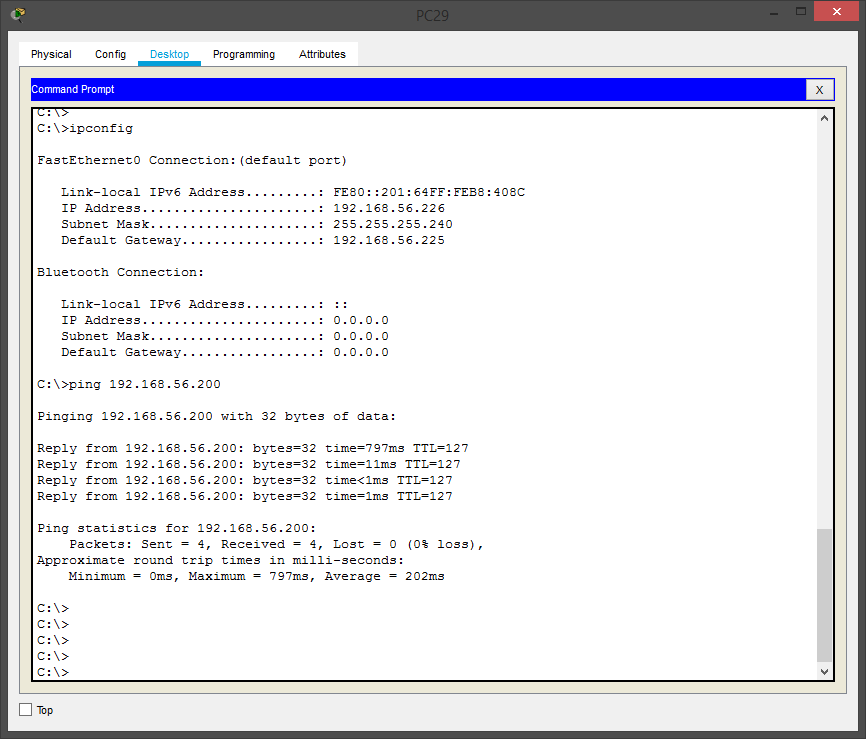
\includegraphics[width = 6 \gridunitwidth]{./assets/09-intervlan-ping.png}
        \caption{Пінг між клієнтами різних віртуальних мереж}
        \label{fig:intervlan-ping}
      \end{figure}

      % Отже, комутатори рівня доступу були правильно налаштовані.

    \subsubsection{Налаштування комутатора рівня розподілу}
      У розробленому проекті комутатор рівня розподілу~— це комутатор рівня~3, який відповідає за підключення і об'єднання комутаторів рівня доступу. Щоб справно виконувати свої задачі, його необхідно налаштувати на роботу зі створеними локальними мережами~(рис.~\ref{lst:switch-l3-trunking}).

      \begin{listingplaintext}{Налаштування комутатора рівня розподілу на підтримку роботи зі створеними віртуальними мережами}{lst:switch-l3-trunking}
        # Увійти в привілейований режим
        en
        # Увійти в режим глобальної конфігурації
        conf t
        # Обрати порти Fast Ethernet 0/1–3
        int range fa0/1-3
        # Налаштуватись на інкапсуляцію транка
        # відповідно до стандарту IEEE 802.1q
        switchport trunk encapsulation dot1q
        # Встановити режим об'єднання в пучок на обраних інтерфейсах
        switchport mode trunk
        # Вказати номери дозволених VLAN
        switchport trunk allowed vlan 2-4
        # Завершити налаштування обраних інтерфейсів
        end
        # Присвоїти IP-адреси створеним VLAN
        int vlan 2
        ip address 192.168.56.193 255.255.255.224
        int vlan 3
        ip address 192.168.56.225 255.255.255.240
        int vlan 4
        ip address 192.168.56.242 255.255.255.240
        exit
        # Увімкнути IP-маршрутизацію
        ip routing
        # Створити VLAN для серверів та мережевого обладнання
        int gi0/1
        switchport mode access
        switchport access vlan 4
        exit
        # Підняти інтерфейси, пов'язані зі створеними VLAN
        int vlan 4
        ip address 192.168.56.242
        vlan 2
        vlan 3
        vlan 4
      \end{listingplaintext}

      Щоб переконатись у правильності налаштувань, необхідно перевірити, чи є підключення від клієнта однієї віртуальної мережі до шлюзу за замовчуванням, який знаходиться в іншій віртуальній мережі~(рис.~\ref{fig:switch-l3-ping}).

      \begin{figure}[!htbp]
        \centering
        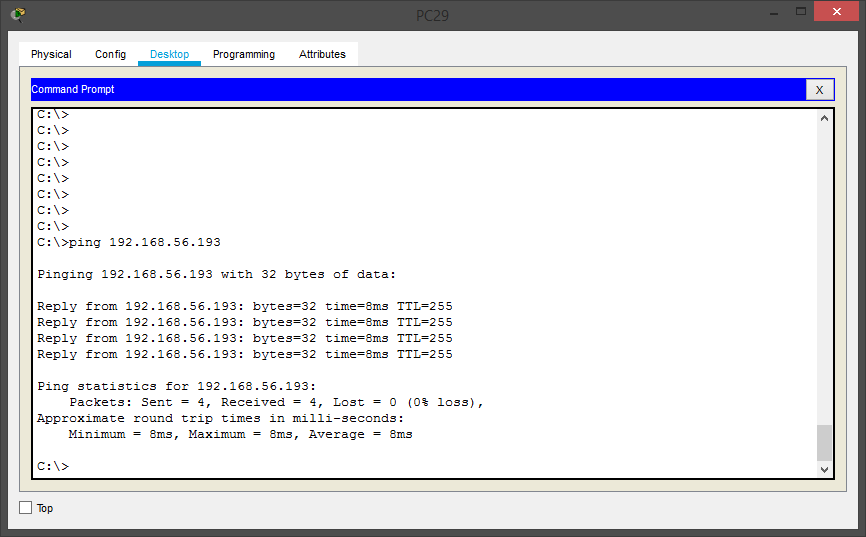
\includegraphics[width = 6.5 \gridunitwidth]{./assets/10-switch-l3-ping.png}
        \caption{Результат перевірки підключення клієнта однієї віртуальної мережі до шлюзу за замовчуванням іншої}
        \label{fig:switch-l3-ping}
      \end{figure}

      Однак, в розробленому проекті мережі, комутатор рівня розподілу відповідає не лише за об'єднання комутаторів рівня доступу, а ще й за розподіл~\textenglish{\allcaps{IP}}-адрес, тому на ньому необхідно налаштувати роботу протоколу~\textenglish{\allcaps{DHCP}}~(лістинг~\ref{lst:switch-l3-dhcp}).

      \begin{listingplaintext}{Налаштування комутатора рівня розподілу на видачу~\textenglish{\allcaps{IP}}-адрес за допомогою протоколу~\textenglish{\allcaps{DHCP}}}{lst:switch-l3-dhcp}
        int vlan 2
        # Створити новий DHCP-пул
        ip dhcp pool DHCP-VLAN2
        # Виділяти IP-адреси із заданої підмережі
        network 192.168.56.192 255.255.255.224
        # Встановити адресу шлюза за замовчуванням для заданого пулу
        default-router 192.168.56.193
        # Встановити адресу DNS-сервера за замовчуванням для заданого пулу
        dns-server 1.1.1.1
        exit
        # Не видавати IP-адресу шлюза за замовчуванням у пулі
        ip dhcp excluded-address 192.168.56.193

        int vlan 3
        ip dhcp pool DHCP-VLAN3
        network 192.168.56.224 255.255.255.240
        default-router 192.168.56.225
        dns-server 1.1.1.1
        exit
        ip dhcp excluded-address 192.168.56.225

        int vlan 4
        ip dhcp pool DHCP-VLAN3
        network 192.168.56.240 255.255.255.240
        default-router 192.168.56.242
        dns-server 1.1.1.1
        exit
        ip dhcp excluded-address 192.168.56.241
        ip dhcp excluded-address 192.168.56.242
      \end{listingplaintext}

      Щоб перевірити правильність налаштувань, необхідно подати запит на~отримання \textenglish{\allcaps{IP}}-адреси від імені одного з клієнтів мережі і перевірити результат. Якщо клієнт отримає адресу і додаткову інформацію, \textenglish{\allcaps{DHCP}}-сервер на комутаторі був правильно налаштовує і наразі працює справно~(рис.~\ref{fig:switch-l3-dhcp}).

      \begin{figure}[!htbp]
        \centering
        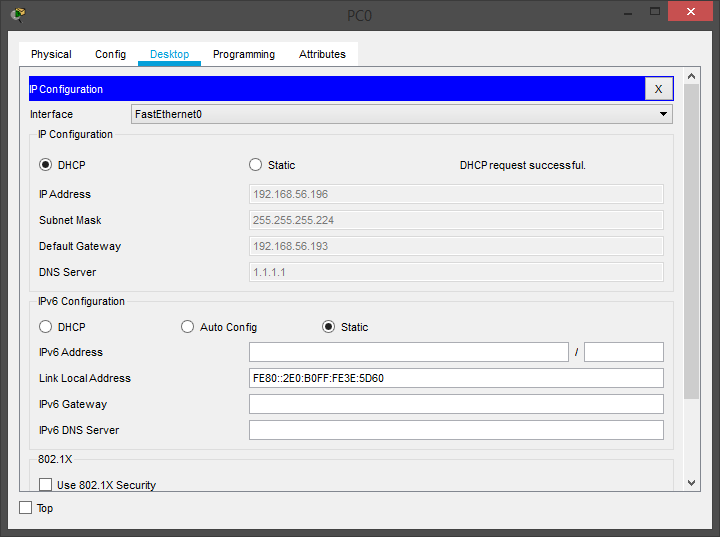
\includegraphics[width = 8 \gridunitwidth]{./assets/11-switch-l3-dhcp.png}
        \caption{Результат запиту клієнта на~\textenglish{\allcaps{IP}-адресу}}
        \label{fig:switch-l3-dhcp}
      \end{figure}

      Після налаштування роботи зі створеними віртуальними мережами, а також видачі~\textenglish{\allcaps{IP}}-адрес клієнтам комутатор рівня розподілу налаштований і готовий до роботи із внутрішньою мережею.

    \subsubsection{Налаштування маршрутизатора}
      Щоб налаштувати маршрутизатор на правильну роботу зі складовими мережі, необхідно налаштувати маршрутизацію у внутрішній мережі, у зовнішній, а також трансляцію мережевих адрес~(лістинг~\ref{lst:router-configuration}).

      \begin{listingplaintext}{Налаштування машрутизатора}{lst:router-configuration}
        # Надати IP-адресу внутрішньому інтерфейсу і включити його
        int gi0/1
        ip address 192.168.56.241 255.255.255.240
        no shutdown
        # Визначити маршрути доступу до внутрішньої мережі
        ip route 192.168.56.192 255.255.255.224 192.168.56.242
        ip route 192.168.56.224 255.255.255.240 192.168.56.242
        ip route 192.168.56.240 255.255.255.240 192.168.56.242
        # Зберегти конфігурацію
        wr mem

        # Налаштувати підключення до роутера провайдера
        int gi0/0
        # Присвоїти надану адресу
        ip address 178.12.46.115 255.254.0.0
        # Увімкнути інтерфейс
        no shutdown
        exit
        # Маршрутизувати увесь невідомий трафік через машрутизатор провайдера
        ip route 0.0.0.0 0.0.0.0 178.12.46.1


        # Налаштування NAT
        ## Визначити зовнішній і внутрішній інтерфейс для перетворення адрес
        int gi0/0
        ip nat outside
        int gi0/1
        ip nat inside

        # Створити список доступу з переліком мереж, які будуть
        # перетворюватись за допомогою NAT
        ip access-list standard FOR-NAT
        permit 192.168.56.192 0.0.0.31 # Wildcard-маски
        permit 192.168.56.224 0.0.0.15
        permit 192.168.56.240 0.0.0.15

        # Визначити правило використання NAT: на інтерфейсі
        # Gigabit Ethernet 0/0
        ip nat inside source list FOR-NAT int gi0/0 overload
      \end{listingplaintext}

      При проведенні вищезазначених налаштувань розуміється, що провайдер надає підключення до мережі інтернет за допомогою власного маршрутизатора з коректними налаштуваннями~(лістинг~\ref{lst:router-isp-conf}).

      \begin{listingplaintext}{Налаштування машрутизатора}{lst:router-isp-conf}
        # Налаштування зовнішнього інтерфейсу, доступного офісній мережі
        int gi0/1
        ip address 178.12.46.1 255.254.0.0
        # Налаштування внутрішнього інтерфейсу, до якого
        # підключений публічний сервер з мережі «Інтернет»
        int gi0/2
        ip address 178.12.47.1 255.254.0.0
      \end{listingplaintext}

      Щоб перевірити правильність виконаних налаштувань, необхідно перевірити підключення до зовнішнього публічного серверу, який знаходиться в симульованій мережі «Інтернет» з комп'ютера внутрішньої мережі. Така перевірка дозволить переконатись не тільки в доступі до мережі~«Інтернет», а й у справній роботі технології~\textenglish{\allcaps{NAT}}. Така перевірка проводиться за допомогою команди~\minttext{ping}~(рис.~\ref{fig:router-ping}).

      \begin{figure}[!htbp]
        \centering
        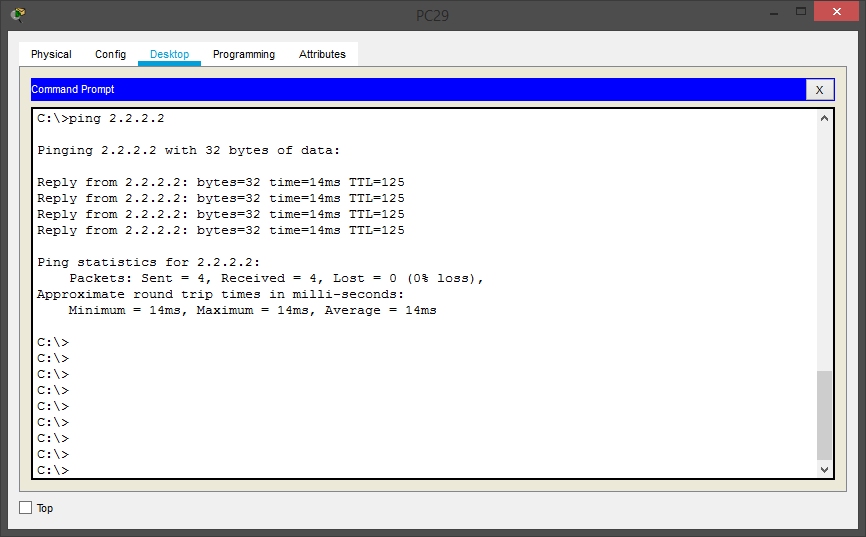
\includegraphics[width = 8 \gridunitwidth]{./assets/12-router-ping.png}
        \caption{Результат перевірки підключення клієнта внутрішньої мережі до публічного сервера в мережі~«Інтернет»}
        \label{fig:router-ping}
      \end{figure}

      Перевірка показала, що кінцевий клієнт має доступ до публічного ресурса мережі~«Інтернет», тому маршрутизатор правильно налаштований, а мережа спроектована і готова до роботи.

  \section*{Висновки}
  \addcontentsline{toc}{section}{Висновки}
  \ESKDthisStyle{nausection}
    Завдання курсової роботи передбачало розробку проекту офісної локальної комп'ютерної мережі. Під час проектування на основі поставлених задач і вимог, а також існуючих теоретичних відомостей були проаналізовані стандартні мережеві топології. Серед проаналізованих топологій була обрана найбільш доцільна~— гібридна деревовидна топологія. Використання деревовидної топології дозволило вправно вирішити поставлені задачі і цілком задовольнити сформульовані вимоги.

    Після вибору топології для проектованої мережі, був описаний план її реалізації, який передбачав вибір необхідного мережевого обладнання і прийняття рішень щодо монтажу мережі. Був проаналізований асортимент мережевих пристроїв, доступний у програмі~\textenglish{Cisco Packet Tracer}, і серед нього обраний найбільш доцільний для реалізації розроблюваного проекту.

    На основі плану фізичної реалізації топології був розроблений план налаштування мережі, в якому був описаний розподіл мережі на віртуальні локальні мережі, схема розподілу~\textenglish{\allcaps{IP}}-адрес у мережі, а також розробка налаштувань для обраного мережевого обладнання. Під час розробки налаштувань мережі були використані такі технології:
    \begin{enumerate}
      \item \textenglish{\allcaps{VLAN}}~— для сегментації мережі.
      \item \textenglish{\allcaps{DHCP}}~— для автоматичної видачі~\textenglish{\allcaps{IP}}-адрес клієнтам.
      \item \textenglish{\allcaps{NAT}}~— для організації коректної роботи кінцевих клієнтів з мережею~«Інтернет».
    \end{enumerate}

    В результаті виконання даної курсової роботи був створений проект офісної локальної комп'ютерної мережі, а розробка цього проекту дозволила отримати і відточити навички проектування локальних комп'ютерних мереж, а також закріпити знання, отримані в ході вивчення курсу~«Комп'ютерні мережі».

  \section*{Список використаної літератури}
  \addcontentsline{toc}{section}{Список використаної літератури}
  \ESKDthisStyle{nausection}
  \begin{litlist}
    \item Болілий В.\,О., Котяк В.\,В. Комп'ютерні мережі. Навчальний посібник. —~Кіровоград: \allcaps{ЦОП}~Авангард, 2008. -~146~с.
    \item Кулаков Ю.\,А., Омельянский С.\,В. Комп’ютерні мережі. Вибір, установка, використання і адміністрування. —~К.: Юніор, 1999. —~544~с.
    \item Гук М. Апаратні засоби локальних мереж. Енциклопедія. —~СПб: Пітер, 2000. —~576~с.
    \item Швиденко М.\,З., Матус Ю.\,В.. Комп’ютерні мережні технології. / Навч.-метод. посібник. —~Київ. —~\allcaps{ТОВ} «Авета», —~2008.
    \item Пістунов І.\,М. Комп'ютерні мережі для спеціалістів з економічної кібернетики: Навч. посібник. —~Дніпропетровськ: \allcaps{НГУ}, 2005. —~125~с.
    \item Гордєєв, О.\,О. Комп’ютерні мережі: навчальний посібник для студентів вищих навчальних закладів / О.\,О. Гордєєв, Д.\,В. Гордєєва, М.\,В. Колдовський; Державний вищий навчальний заклад «Українська академія банківської справи Національного банку України». —~Суми: \allcaps{ДВНЗ} «\allcaps{УАБС НБУ}», 2011. —~250~с.
    \item Машкаров Ю.\,Г. Комп’ютерні мережі та телекомунікації: навч. посіб. Ю.\,Г.~Машкаров. I.\,В.~Кобзев. О.\,В.~Орлов. М.\,В.~Мордвинцев. —~X. Внд-во Хар\allcaps{РГ} \allcaps{НАДУ} «Магістр», 2012. —~212~с.
  \end{litlist}

\end{document}
